%!TEX root = ../thesis.tex
\section{Background}
\paragraph{}
The Finite element method (FEM) constitutes a general tool for the numerical solution of partial differential equations in engineering and applied science \citep{Ucb2010}.
It did not achieve enormous popularity until early 1950s, when digital computer was developed.
After that, the method was refined with the help of variational methods from Lord Rayleigh (1870) and W. Ritz (1909) as well as the Galerkin's weighted-residual approach \citep{Fel1994}.
Then, great amount of research has been conducted on the FEM in terms of mathematics and applications, contributing to its dominance over numerical method in solid mechanics and structural analysis by the beginning of the 1990s \citep{Clo1980}.
Although it is a principle method for solving complex problems in the engineering field, deficiency in geometric representation has been detected.
Besides, inability to formulate unbounded domain restricts the FEM in some area.

\paragraph{}
In the existing computational methods, the geometry is interpolated by high order polynomials and the exact geometry is neglected due to its intricacy. However, the accuracy of adopting it into computational mechanics seems to be limited \citep{Sza2004}.
Convergence study (Fig.~\ref{intro_fig:geolimit}) exhibits the inability for error to decrease at some level with an increasing order.
In Fig.~\ref{intro_fig:geolimit2}, there is hardly any difference in results between the order of $4$ and $8$.
That proves the geometric error cannot be prevented by the elevation of order.
Besides, low-order elements are used widely in finite element analysis which increases the error from geometry.
%
\begin{figure}
    \centering
    \scalebox{0.8}{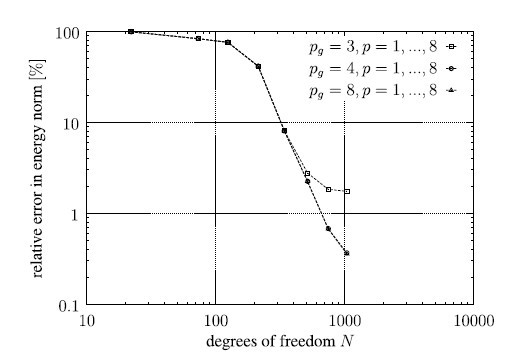
\includegraphics{introduction/img/geolimit.jpg}}
    \caption[Accuracy limit in Scordelis-Lo roof problem]{Convergence study of the Scordelis-Lo roof problem: $p_g$ stands for the order of the polynomial used to represent the geometry, $p$ is order of the polynomials adopted in structural analysis \citep{Ran2005}}
    \label{intro_fig:geolimit}
\end{figure}
%
Geometrical imperfection can lead to imprecise estimates. This is shown by comparing the buckling load.
Error from geometric imperfection swells significantly in Fig.~\ref{intro_fig:geolimit2}.
%
\begin{figure}
    \centering
    \scalebox{0.6}{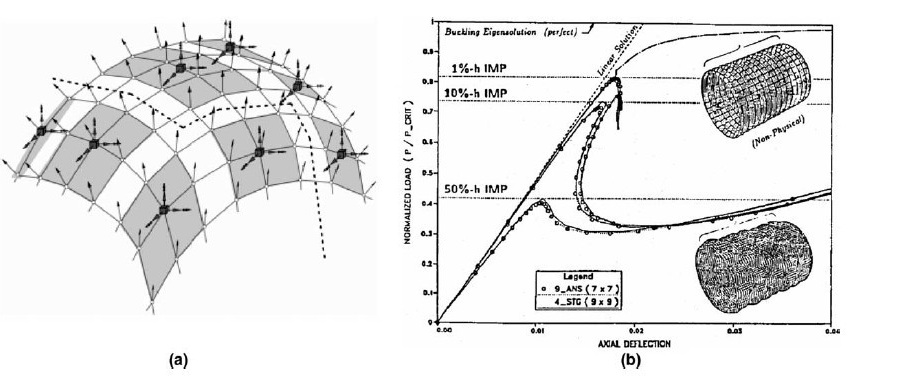
\includegraphics{introduction/img/imp.jpg}}
    \caption[Thin shell shows considerable geometric sensitivity]{Thin shell shows considerable geometric sensitivity: (a) error in geometric representation generated in a typical finite element analysis \citep{Gee2005} (b) buckling load of cylindrical shell with geometric imperfections \citep{Sta1985}}
    \label{intro_fig:geolimit2}
\end{figure}
%
\paragraph{}
Tensor product Non-Uniform Rational B-spline (NURBS) is a well-known curve and surface representation method and has been adopted as a standard in computer graphics, computer-aided-design (CAD) \citep{Nas2003} and Initial Graphics Exchange Specification (IGES) since 1983 \citep{IGES1983}.
Nowadays, the employment of rational polynomial functions in description of geometry in CAD/CAM applications is becoming more and more extensive \citep{Pie1987}.
A general sculptured surface can be built easily with the help of NURBS \citep{Rog2001}.
One of its strongest reasons for that is its ability to represent any conic curves and surfaces precisely.

\paragraph{}
The reason why the geometry is represented differently in computer aided design (CAD) and finite element analysis is because of the different time they were born.
Commercial software with the FEM has already been designed by the late 1960s and it spread to other engineering fields due to its convenience and accuracy.
It employs variational methods (the Calculus of variations) to minimize the error function in order to achieve a converge solution.
However, CAD, which gives an exact description on geometry, has not been developed until 1980s \citep{Dav2008}.
The first Unigraphics System (for 2D modelling and drafting) was sold by United Computing in 1975 \citep{Ste2010}.
Nowadays, CAD has been widespread and won even more popularity than finite element analysis does.
While, the geometric descriptions adopted by engineers today for CAD and that for analysis are totally different.
One rough estimate provided by \cite{Hug2005} suggests that more than half of the overall analysis time is spent on meshing in the industries such as automotive and aerospace where complex shapes are involved.
Furthermore, frequent design modifications in fast pace, modern society restricts the usage of analysis if a new mesh cannot be created in a short duration.

\paragraph{}
Creation of mesh in FEM can be expensive in terms of time and human resource.
One possible solution is trying to replace the geometric modelling tool in FEM by something more CAD-like.
NURBS, for example, is a standard mathematical model utilized in CAD industry.
Exact CAD geometric boundary is achieved with the help of the NURBS curve and surface.
This idea to be geometrically exact with a minimum discretization is adopted in Isogeometric analysis developed in 2005 \citep{Hug2005b} and further refined recently \citep{Zhang2007,Hug2005b,Cot2006,Cot2009,Baz2006a,Baz2006b}.
Furthermore, a simplified mesh refinement method by omitting the necessity for communication with the CAD geometry once the initial shape is received is also targeted \citep{Cot2007}.
It shows advantage in the structure analysis (Fig.~\ref{intro_fig:thinshell}), fluid mechanics \citep{Buf2011} and dynamics (Fig.~\ref{intro_fig:Femvsnurbs}).
%
\begin{figure}
    \centering
    \scalebox{0.7}{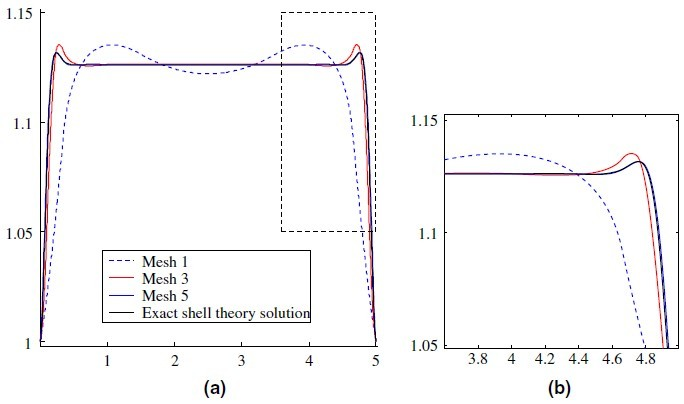
\includegraphics{introduction/img/thincylindricalshell.jpg}}
    \caption[Thin cylindrical shell]{Thin cylindrical shell. Convergence study of radial displacement (a) global displacement  (b) boundary layer \citep{Hug2005}}
    \label{intro_fig:thinshell}
\end{figure}
\begin{figure}
    \centering
    \begin{subfigure}[b]{0.49\linewidth}
        \centering
        \scalebox{0.4}{
            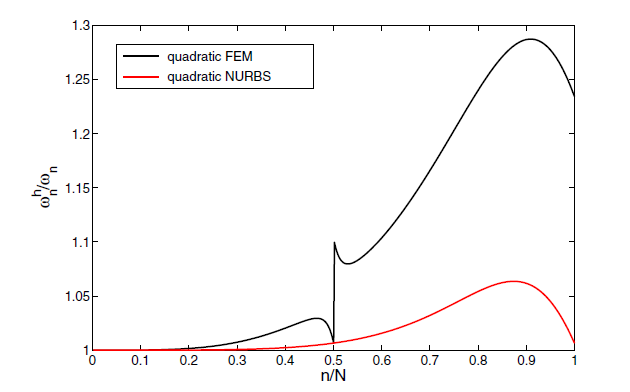
\includegraphics{introduction/img/Femvsnurbs.png}
        }
    \end{subfigure}
    \begin{subfigure}[b]{0.49\linewidth}
        \centering
        \scalebox{0.43}{
            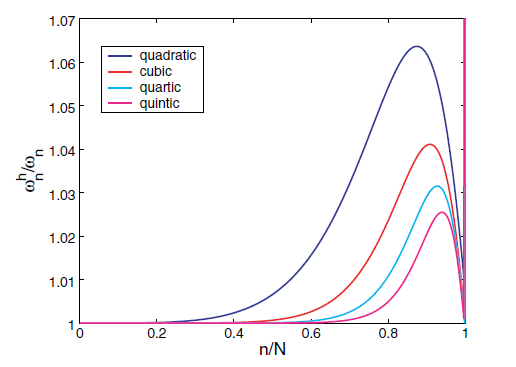
\includegraphics{introduction/img/order.png}
        }
    \end{subfigure}
    \caption[Normalized discrete spectra]{(a) Normalized discrete spectra \citep{Cot2006}. (b) different order of NURBS basis functions. Outliers appear in the very thin band on the right end of the spectrum}
    \label{intro_fig:Femvsnurbs}
\end{figure}



%  ------------------------------------------- %
\section{State of the problem}
\label{intro_sec:problem}
\paragraph{}
In current Isogeometric analysis, accuracy problems with numerical integration of a rational polynomials attract significant attention \citep{Hug2010,Sev2011,Aur2012}.
Furthermore, incapability to create a set of control points to fit an inhomogeneous essential boundary condition may lead to considerable errors and lower converge speed due to the non-interpolatory characteristics of the NURBS surface and curves \citep{Wang2010,Wol2011,Koo2013}.
Besides, although numerous amount of research has been conducted on improving the algorithm efficiency \citep{Boo1972,Qin1996,Cho1990,Gra1992,Pan2001,Wang2012}, most of the time is devoted to calculate the basis function which restricts the usage of high order basis function in 3D problems.
Moreover, one of the most critical problems in the existing Isogeometric analysis lies in dimension incompatibility.
It is based on FEM where 3D NURBS solids are required for meshing in 3D problems but only the boundary is described in CAD system.
Further meshing process for converting input surface data to higher dimension physical geometry in isogeometric analysis has been referred to as ``analysis-aware modelling'' \citep{Coh2010}.
Considerable research on solving this incompatibility by domain parameterization has been performed using a variety of methods \citep{Yang2007,Aig2009,Mar2009,Qian2011}.

% qudatree and octree
\paragraph{}
In order to eliminate the need for domain parameterization, a NURBS based Boundary Element Method (BEM) is proposed \citep{Li2011,Taka2012,Beli2013,Sco2013,Sim2013}.
In BEM, only the boundary was discretised, contributing to a reduction of the spatial dimension by one and hence be fully compatible with CAD output geometric data. Moreover, error induced in boundary condition fitting and numerical integration decreases and higher order basis function can be utilized to achieve higher accuracy. Nevertheless, the fundamental solution satisfying the governing differential equations in the domain must be available.
Unfortunately, this fundamental solution may be extremely complex.
A Scaled Boundary finite element method (SBFEM) which has similarity with both the FEM and the BEM is proposed to eradicate the necessity of fundamental solution in BEM.
SBFEM is a novel semi-analytical approach developed by Wolf and Song \citep{Wol1999}.
As a method developed based on FEM and BEM, SBFEM is a fundamental-solution-less boundary element method which keeps the benefits of the both as well as provides some effective solutions to the limitations to the FEM and the BEM \citep{Wol1999}.
The fundamental solution is no longer required, spatial dimension is reduced by one as only the boundary is meshed with surface elements which lead to decline in the number of unknowns and achievement of infinite boundary \citep{Wol2003}.
However, like the conventional FEM, a meshing process which could be expensive in terms of human resource is required in the SBFEM as well.
Besides, as a numerical method based on meshing, the quality of the mesh may significantly influence the accuracy of the result.
Consequently, it could be necessary to develop automatic mesh generation algorithms that can produce high quality scaled boundary finite element with achieving conforming boundary recovery in both 2D and 3D problem in order to reach a systematic and automatic numerical method that requires minimal human involvement.

% adaptive mesh refinement
\paragraph{}
% The accuracy of the result calculated by SBFEM is highly relevant to the mesh quality.
Mesh refinement is a common process during numerical analysis to improve the accuracy and ensure the result is converging.
A naive uniform refinement may lead to not only over-refined in area contributes few to the improvement of the accuracy which can be computationally inefficiency but also under-refined which results the omission of localized phenomena.
This motivates the idea of adaptive mesh refinement which try to determine whether an element need refined based on a ``posteriori error estimator''.
Numerous research has been conducted on such an error estimator and it has been developed in the FEM \citep{Duval2018, doi:10.1002/gamm.201490020,PRUDHOMME20091887}, the BEM \citep{Zhao1998, Guiggiani1990, KAMIYA1992223} and the SBFEM \citep{NME:NME439}.
However, some of these error estimator requires extra work such as stress recovery.
Besides, it could be difficult to determine the most suitable error indicator to a given problem.
Furthermore, the threshold is taken manually which limits the usage of several indicators as the number of the threshold grows quadratically as the number of the estimators increases.



%  ------------------------------------------- %
\section{Objective and significance}
\paragraph{}
As discussed in Sec.~\ref{intro_sec:problem}, there are several limitations associated with the existing numerical methods.
This thesis aims at developing a complete and systematic numerical method where all procedures are conducted without human involvement for an arbitrary geometric input in both 2D and 3D situations.
After the design files (IGES file and STL file in 3D) are delivered in electronic form, the proposed method shall be able to parse the geometric input, generate the mesh (quadtree in 2D and octree in 3D), determine the result using SBFEM and refine the mesh based on the error estimator automatically.
The main objectives of this thesis are as follows
\begin{enumerate}
    \item Minimize human effort spent on engineering mechanics analysis
    \item Be compatible with arbitrary geometric input in 2D and 3D
    \item Generate high quality mesh
    \item Retain exact geometry
    \item Develop a robust, extensible and flexible error estimator
\end{enumerate}
Accomplishing tasks mentioned above makes significant contributions to solve the practical engineering problems automatically.
Furthermore, a new error estimator trained using machine learning algorithm allows unlimited number of indicators to be used.

%  ------------------------------------------- %
\section{Outline of the thesis}
\paragraph{}
In the next chapter, a literature review on the existing numerical methods including Isogeometric analysis and SBFEM, automatic mesh generation algorithm and adaptive mesh refinement is presented.
The advantages and disadvantages of different methods are critically discussed.

\paragraph{}
In Chapter 3, the idea of the isogeometric analysis is extended to the SBFEM to solve 2D problem including linear elasticity and linear elastic fracture mechanics.
The NURBS basis functions are adopted as the shape functions in the SBFEM instead of the conventional Legendre polynomials.
Some key formulation in linear elasticity and linear elastic fracture mechanics in SBFEM using NURBS shape functions are derived.
In order to perform a numerical integration on piecewise polynomials, a knot insertion is adopted to convert a piecewise polynomials to multiple traditional polynomials.
NURBS curve fitting is also introduced to enforce the stress boundary condition.

\paragraph{}
Chapter 4 implements IGES adaptor which can convert the geometric information stored in IGES file into polylines.
A quad-tree based mesh generation algorithm is also developed to handle arbitrary geometric input from AutoCAD.
In order to retain the exact geometry, the intersection point is projected back onto the original NURBS curve.
The projection is improved using the convex hull property and the quick hull algorithm is hence introduced.
Hard point is introduced in order to handle the multiple material interfaces, sharp edges or crack.
Optimization algorithms such as bucket sort is adopted to improve the computational efficiency for the mesh generation.
Stress analysis is conducted on 2D linear elasticity problems.

\paragraph{}
In Chapter 5, an adaptive mesh refinement algorithm is proposed by the help of machine learning.
Expressions related to the eigenvalues of the SBFEM formulation together with some key geometric properties of the scaled boundary finite element are obtained as the error indicators.
The models trained by Multilayer Perceptron (MLP), Support Vector Machine (SVM) using radial kernel function and random forest are compared to each others and the model that achieve the best performance (MLP) is used as the final one.
In order to improve the learning effectiveness of the MLP, regularization methods including bagging and dropout are adopted.
Due to the lack of eigenvalue error indicator in first order triangular element, method that eliminates these situation is produced.
A matrix representation of NURBS curves is presented to achieve a higher efficiency and stability in calculating the intersections between lines and NURBS curve.
Stress analysis is conducted on 2D linear elasticity problems.

\paragraph{}
Chapter 6 develops a method that can project intersection points from an octree 3D SBFE mesh back to their origin NURBS surfaces in order to retain the exact geometry.
Splitting of NURBS surfaces are introduced to accelerate the algorithm in both point projection and intersection calculation.
The computational efficiency of them are further improved by utilizing the strong hull properties of the NURBS surface and hence the quick hull algorithm in 3D is introduced.
Another method to keep the exact geometry is calculating the intersection between lines and NURBS surfaces instead of performing the projection.
The matrix representation of NURBS surfaces in 3D is introduced to improve the computational efficiency and stability of the calculation of the intersection.



\paragraph{}
Chapter 7 presents conclusions to the research.
Possible future works are proposed.